\documentclass[a4paper]{article}
\usepackage[utf8]{inputenc}

% Author affiliation
\usepackage{authblk}
% Package for line spacing
\usepackage{setspace}
\renewcommand{\baselinestretch}{2.0} % Double spacing
% Margins
\usepackage[margin=1.25in]{geometry}
% Mathematics
\usepackage{amsmath}
% Tables
\usepackage{tabularx}
\usepackage{booktabs}
% SI units
\usepackage{siunitx}
% Links and referencing within the document
\usepackage[backref]{hyperref}
\hypersetup{hidelinks} 
% Advanced math typesetting
\usepackage{mathtools}
% Graphics
\usepackage{graphicx}
\usepackage{subfig} 
\graphicspath{{./figures}} % Adjust path as needed

\title{This is only an example}

\author[1$\dag$]{X}
\author[1$\dag$]{H}
\author[1*]{Q}
\author[1,2]{S}

\affil[1]{School of R, China}
\affil[2]{School of A, China}
\affil[*]{Address correspondence to: email}
\affil[$\dag$]{These authors contributed equally to this work.}

\begin{document}

\maketitle

\begin{abstract}
Reconfigurable battery systems provide a promising alternative to traditional battery systems due to their flexible and dynamically changeable topological structures that can be adapted to different battery charging and discharging strategies.
...
\end{abstract}

\section{Methodology}

The central principle of the proposed method is to connect the batteries in an RBS in parallel to the maximum possible extent, thereby maximizing the output current.
To achieve this universally and automatically, the overall process is divided into the four steps shown in Fig. \ref{fig:main}.
...

\begin{figure}[htbp]
    \centering
    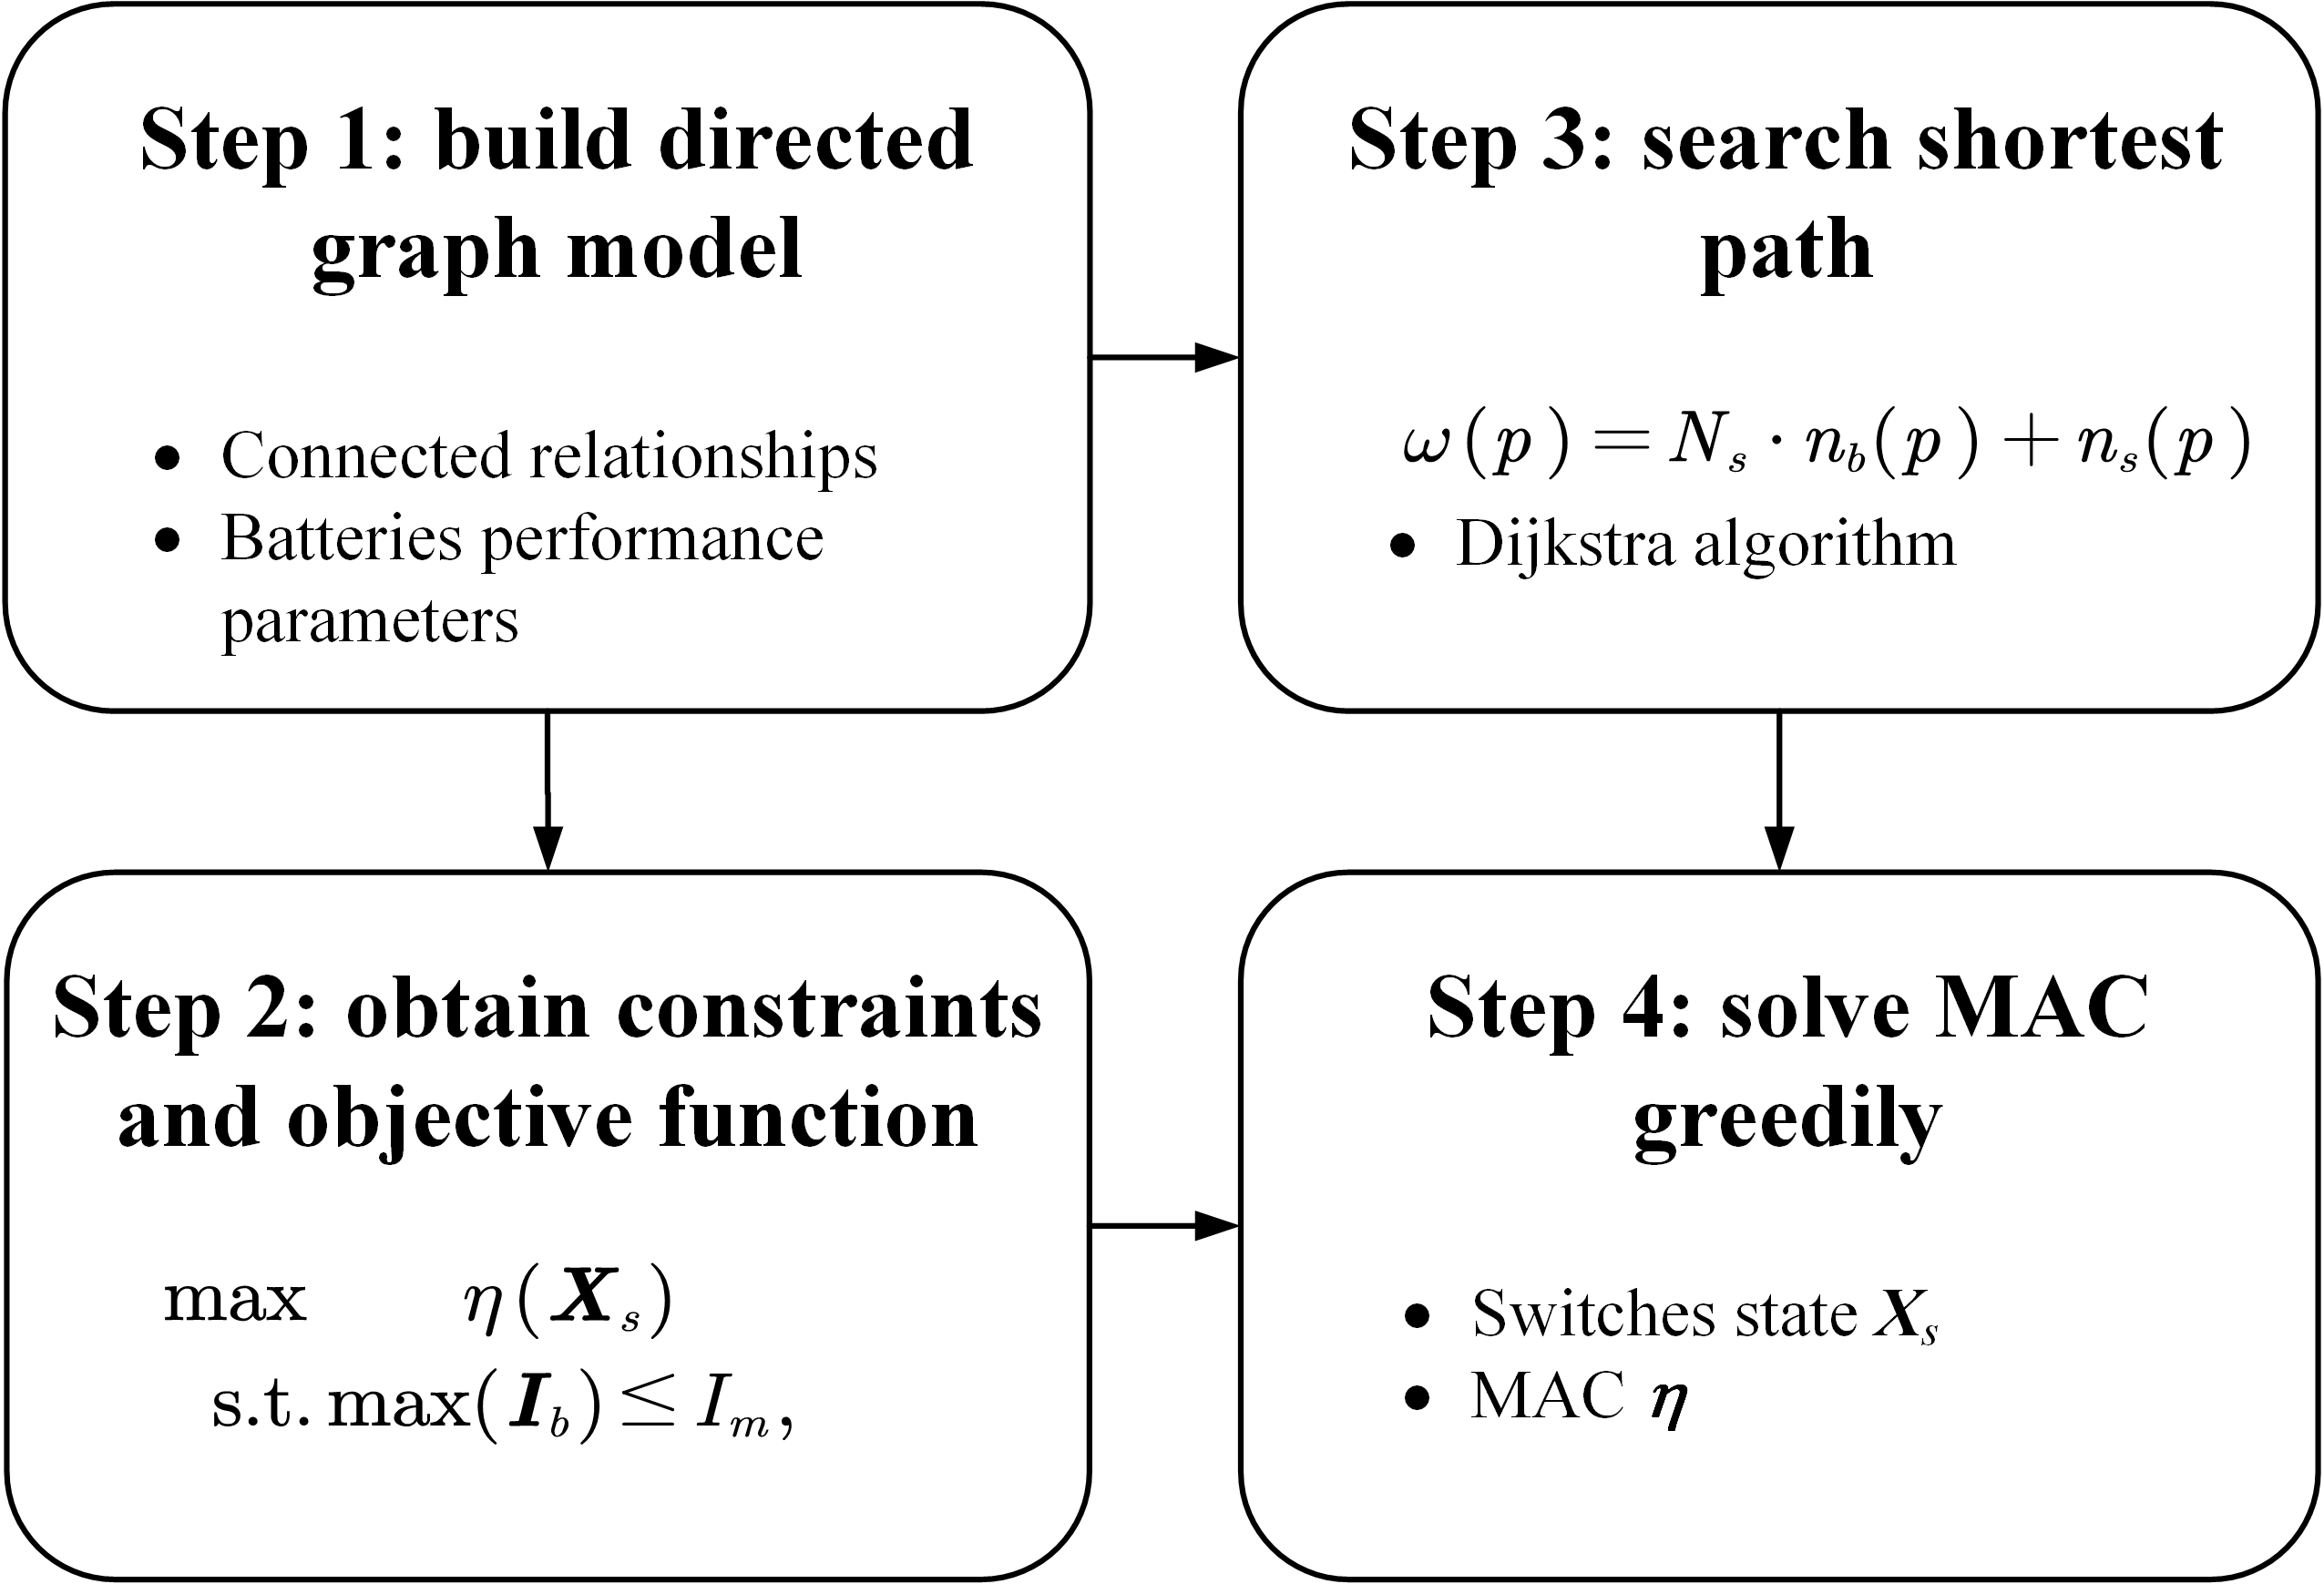
\includegraphics[width=0.8\linewidth]{main.png}
    \caption{
        A diagram of the proposed method, which contains four main steps.
    }
    \label{fig:main}
\end{figure}

\subsection{Directed graph Model}

\begin{figure}[htbp]
    \centering
    \subfloat[]{
        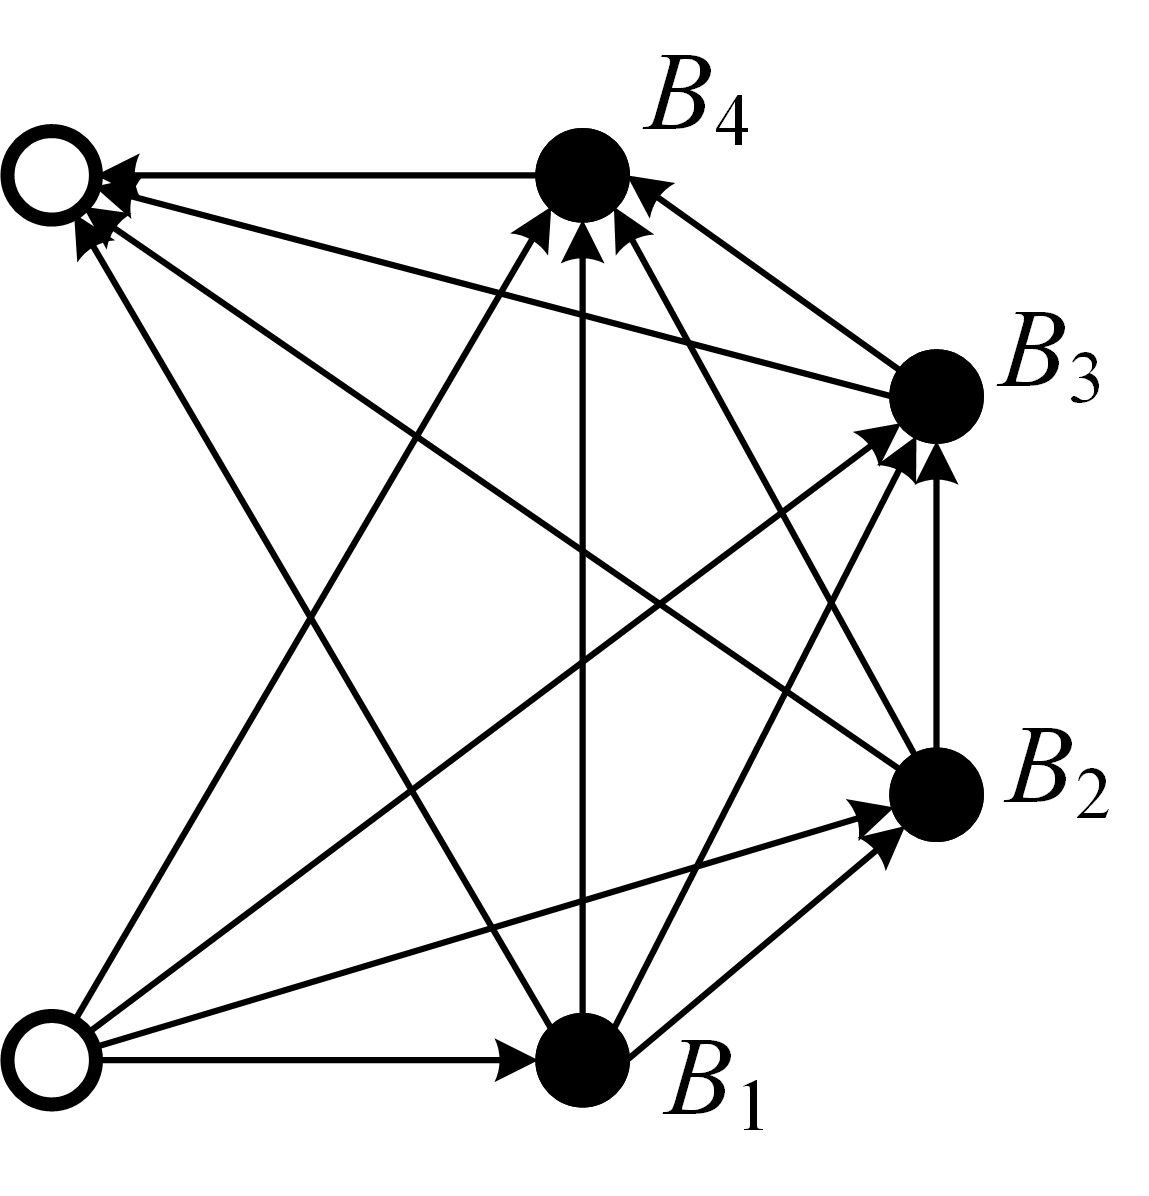
\includegraphics[width=0.31\linewidth]{direct-graph-he.png}
    }
    \subfloat[]{
        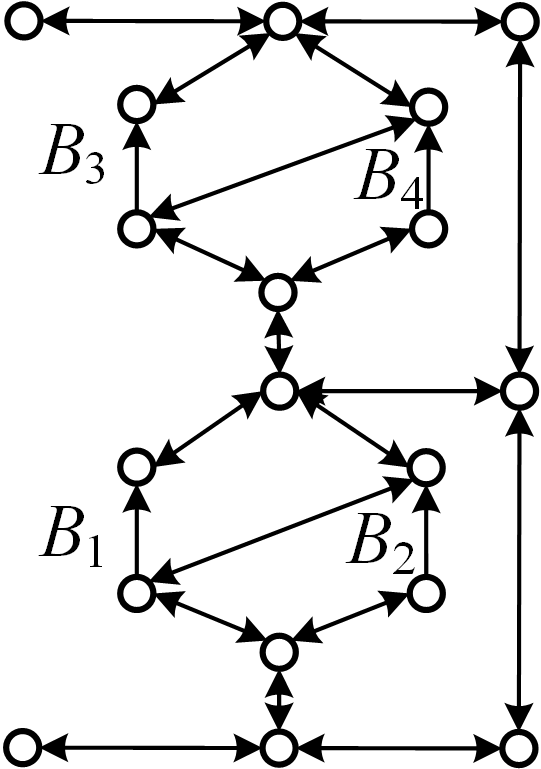
\includegraphics[width=0.23\linewidth]{direct-graph-xu.png}
    }
    \subfloat[]{
        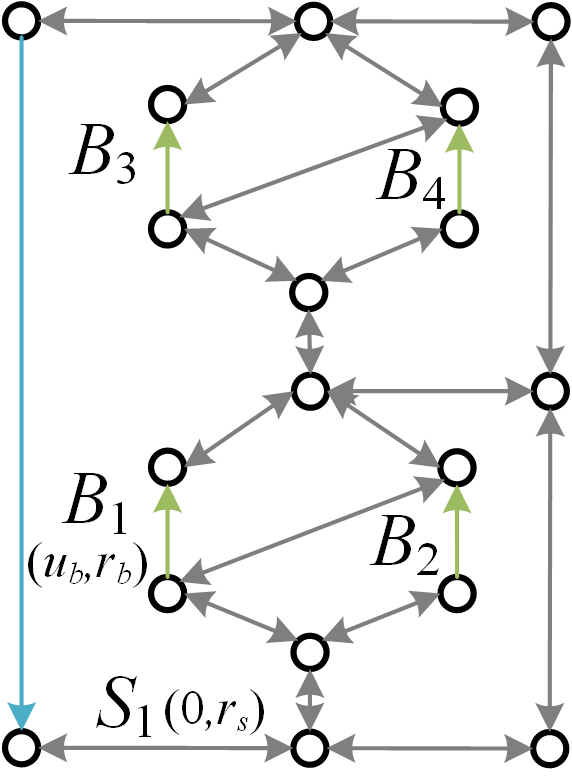
\includegraphics[width=0.24\linewidth]{direct-graph-my.png}
    }
    \\
    \subfloat[]{
        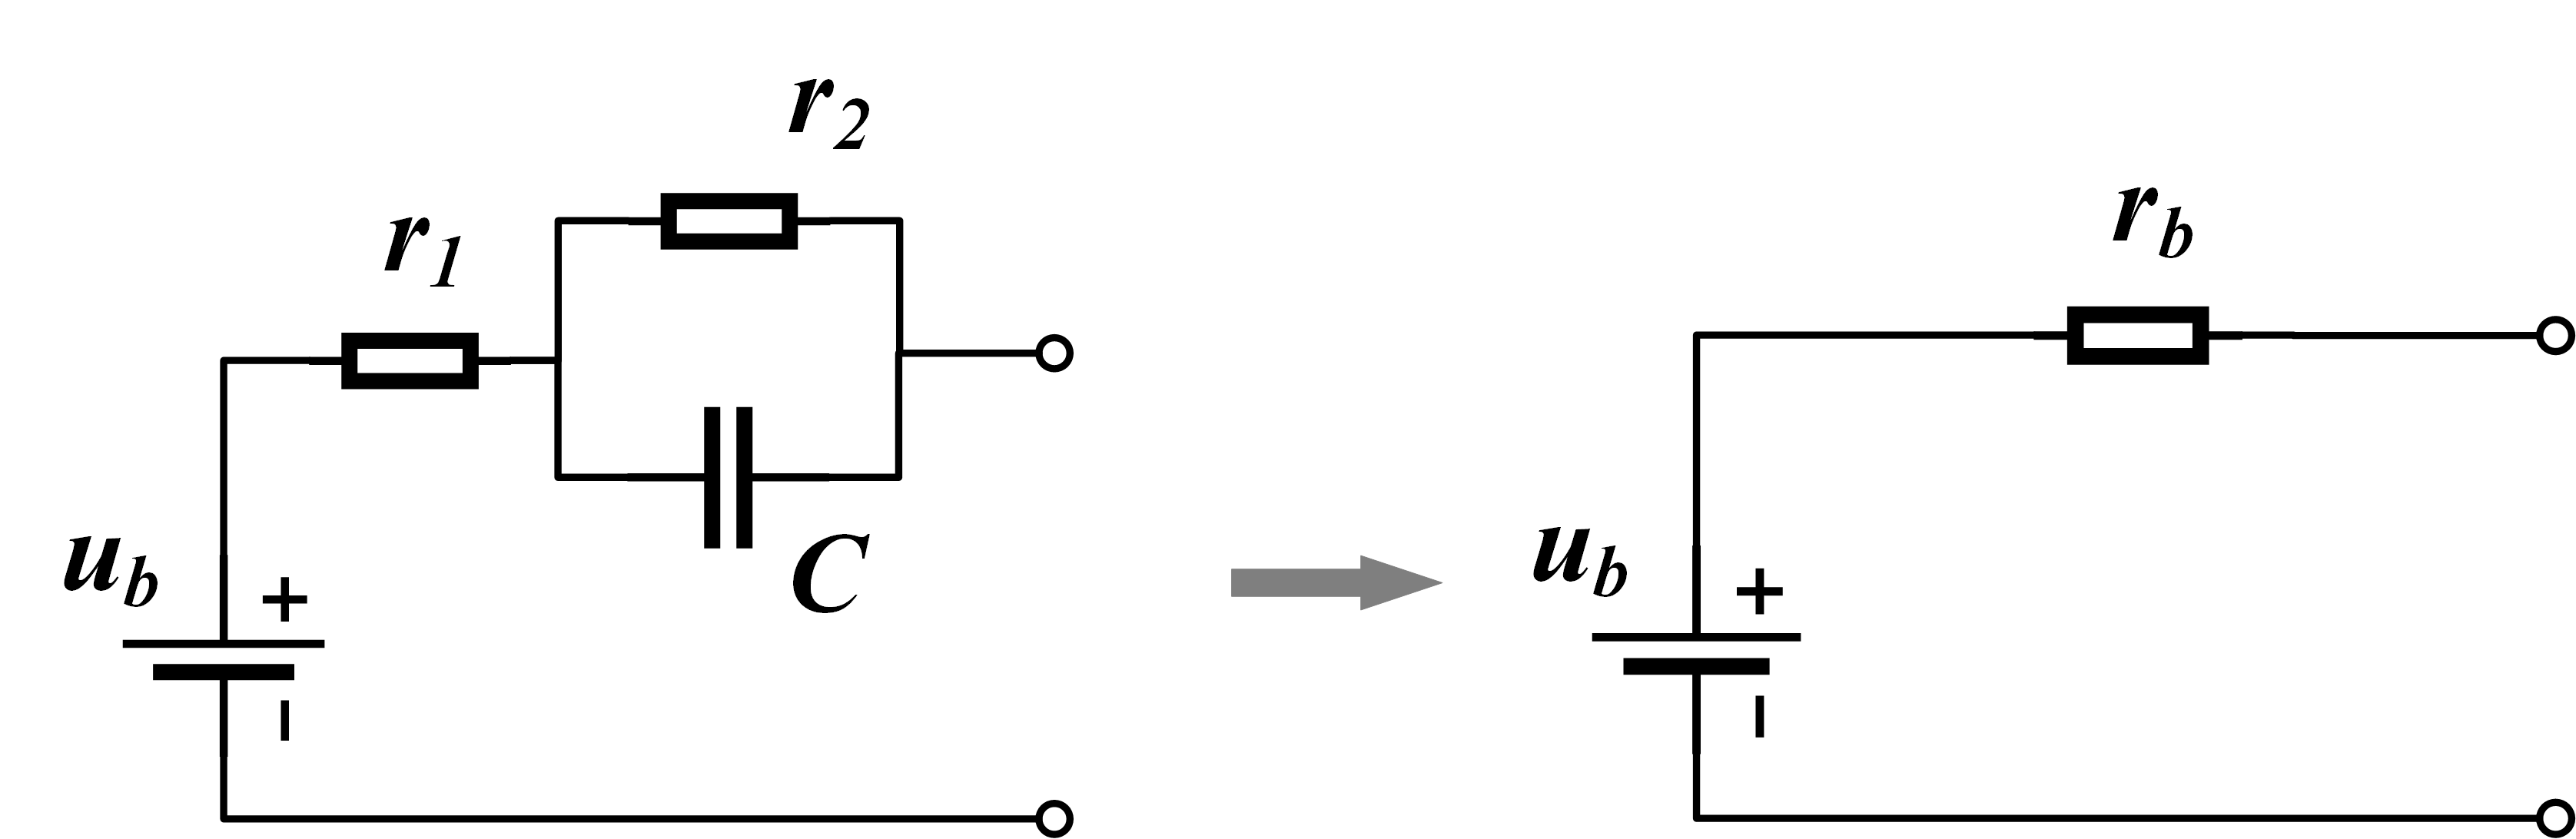
\includegraphics[width=0.8\linewidth]{battery_simple.png}
    }
    \caption{
        The directed graph models used in (a) the work of He et al. \cite{heExploringAdaptiveReconfiguration2013}, (b) our previous work, and (c) the improved model in this paper.
        (d) The equivalent circuit of a battery in this method.
    }
    \label{fig:model}
\end{figure}

% He et al. \cite{heExploringAdaptiveReconfiguration2013} proposed an abstracted directed graph model for an RBS, where the nodes represent the batteries, the edges represent the configuration flexibility, and the weight of each vertex corresponds to the battery voltage (Fig. \ref{fig:direct-graph-he}). 
% The model captures all potential system configurations and offers a direct metric for configuration flexibility, but it does not specify the physical implementation of the connectivity between batteries, meaning that one graph might correspond to multiple RBS structures.
% We previously proposed a directed graph model that differs significantly from He et al.'s model by using nodes to represent the connections between batteries and switches and directed edges to represent batteries and switches (Fig. \ref{fig:direct-graph-xu}), allowing for a one-to-one correspondence between an RBS structure and its directed graph model. 
% ...
% The model also considers the external load as an equivalent resistance and integrates it into the analysis, making it a complete circuit model for later circuit analysis.
% Fig. \ref{fig:direct-graph-my} shows the improved directed graph model used in this paper.
% The following provides a detailed explanation of the method used for equating components in RBSs and constructing the directed graph model.

He et al. \cite{heExploringAdaptiveReconfiguration2013} proposed an abstracted directed graph model for an RBS, where the nodes represent the batteries, the edges represent the configuration flexibility, and the weight of each vertex corresponds to the battery voltage (Fig. \ref{fig:model}(a)). 
...
We previously proposed a directed graph model that differs significantly from He et al.'s model by using nodes to represent the connections between batteries and switches and directed edges to represent batteries and switches (Fig. \ref{fig:model}(b)), allowing for a one-to-one correspondence between an RBS structure and its directed graph model. 
...
Fig. \ref{fig:model}(c) shows the improved directed graph model used in this paper.
The following provides a detailed explanation of the method used for equating components in an RBS and constructing the directed graph model.


\subsection{Constraints and Objective Function}

First, the topology in the directed graph model is represented in the form of a matrix $\boldsymbol{A}$, which is known as the incidence matrix and is defined as Eq. \eqref{eq:A}:
\begin{align}\label{eq:A}
    a_{kl}=
    \begin{cases}
        1,  & \text{edge $l$ leaves node $k$},\\
        -1, & \text{edge $l$ enters node $k$},\\
        0,  & \text{otherwise}.
    \end{cases}
\end{align}
For a directed graph consisting of $N$ nodes and $N_b+2N_s+1$ directed edges, the incidence matrix $\boldsymbol{A}$ is an $N\times(N_b+2N_s+1)$ matrix. 
In this matrix, the rows and columns represent the nodes and edges of the directed graph, respectively.
By distinguishing the components in the RBS corresponding to each column, $\boldsymbol{A}$ can be rewritten as
\begin{equation}\label{eq:A_bso}
    \boldsymbol{A} =
    \begin{bmatrix}
        \boldsymbol{A}_b & \boldsymbol{A}_s & \boldsymbol{A}_o
    \end{bmatrix},
\end{equation}
where $\boldsymbol{A}_b$, $\boldsymbol{A}_s$, and $\boldsymbol{A}_o$ are the sub-matrices corresponding to the batteries, switches, and external electrical load, respectively.
...
Thus, for the sub-matrix $\boldsymbol{A}_s$, only one column is retained for each pair of columns representing the same switch.
...
Similar to Eq. \eqref{eq:A_bso}, $\boldsymbol{\tilde{A}}$ can be rewritten as
\begin{equation}\label{eq:A_bso_tilde}
    \boldsymbol{\tilde{A}} =
    \begin{bmatrix}
        \boldsymbol{\tilde{A}}_b & \boldsymbol{\tilde{A}}_s & \boldsymbol{\tilde{A}}_o
    \end{bmatrix}.
\end{equation}

\bibliographystyle{ieeetr}
\bibliography{../ref}

\end{document}
